\chapterimage{lan_party.jpg}
\chapter{Layer 2: Network (LAN) communication}\label{sec:layer2}

\begin{minipage}{0.4\linewidth}
\begin{center}
\begin{bytefield}{16}
\bitbox{16}{Layer 7: Application} \\
\bitbox{16}{Layer 4: Transport} \\
\bitbox{16}{Layer 3: Internet} \\
\bitbox{16}{\color{color1} Layer 2: Network (LAN)} \\
\bitbox{16}{Layer 1: Physical} \\
\end{bytefield}
\end{center}
\end{minipage}
\begin{minipage}{0.6\linewidth}
\begin{center}
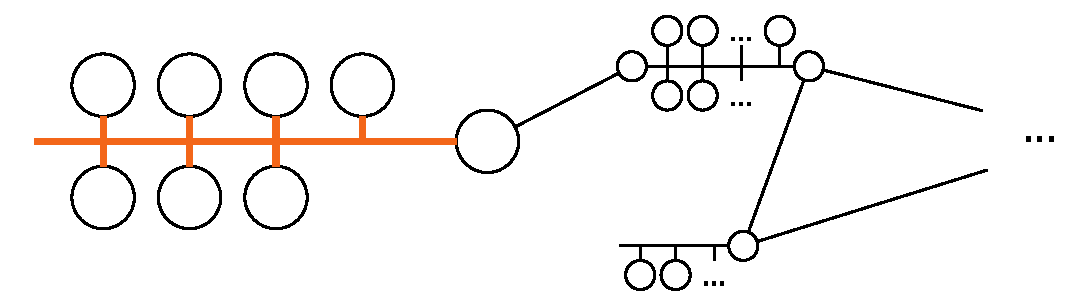
\includegraphics[width=\linewidth]{network_layer2.pdf}
\end{center}
\end{minipage}

\vspace{-0.75cm}

% \section{Layer~2 overview}
\subsection*{Capabilities}

Layer~2 protocols allow multiple devices to exchange messages
and identify each other within a local network (\concept{LAN}).
% 
Devices outside the LAN cannot be contacted \textit{directly} with Layer~2 protocols.

Layer~2 abstracts upper layers (including user applications) from the specifics of connected hardware.
This makes it easier (read: cheaper) to write code once and run it everywhere.

Layer~2 messages are limited in length. The maximum amount of Payload data 
that can be inserted in a Layer~2 protocol is called the \conceptRef{MTU}{Maximum Transmission Unit (MTU)},
\eg, $1500$~bytes for Ethernet.

Some Layer~2 protocols may also provide user \concept{authentication} and
\conceptRef{cryptography}{cryptographic} protection; 
\concept{Wi-Fi} is a notable example,
although wired networks may also employ, \eg, IEEE 802.1X.

\vspace{-0.3cm}
\begin{center}
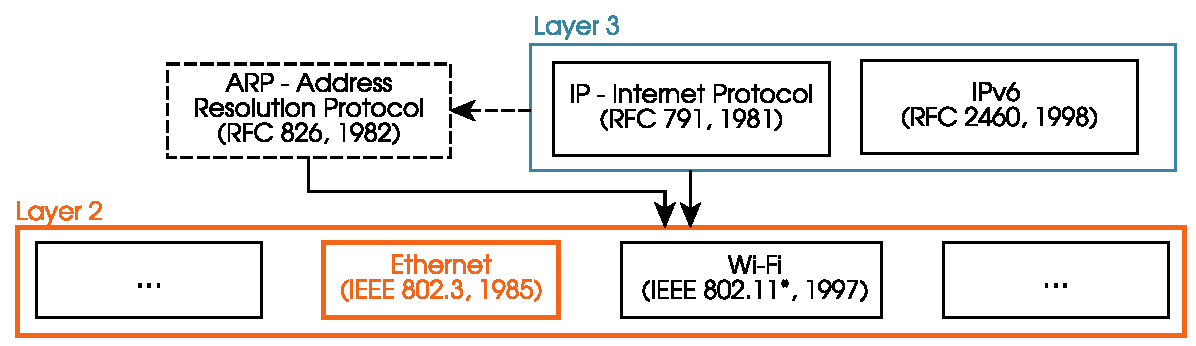
\includegraphics[width=0.9\linewidth]{protocols_layer2.pdf}
\end{center}
\vspace{-0.5cm}

\subsection*{Protocols}
Many \concept{protocols} have been and are being defined within Layer~2. Most importantly nowadays:\\[-0.65cm]
\begin{itemize}
\item \concept{Ethernet} (IEEE 802.3), addressed in \secref{sec:layer2:ethernet}.
\item \concept{Wi-Fi} (\eg, IEEE 802.11be aka Wi-Fi 7, of 2024).
\end{itemize}

Within \concept{TCP/IP}, Layer~2 \conceptRef{encapsulation}{encapsulates} the following protocol \conceptRef{PDU}{PDUs}
(both addressed in Chapter~\ref{sec:layer3}):\\[-0.65cm]
\begin{itemize}
  \item \concept{IPv4} and \concept{IPv6} \conceptRef{datagram}{datagrams}.
  \item \concept{ARP} messages.\\[-0.75cm]
\end{itemize}

\vspace{0.5cm}

\begin{remark}
The \inlineCode{ip link} command shows and can configure your interfaces,
including the \concept{MAC} address.

Your Operating System typically assigns internal interface names automatically based on their type,
\eg, \inlineCode{eth0} or \inlineCode{wlan1}.
% 
Interfaces can usually be renamed, because interface names 
are not part of TCP/IP; they are used exclusively within that Operating system.
\end{remark}


\section{Layer~2 addressing}
In most LAN technologies, Layer~2 addresses are numeric IDs unique for each device within the LAN. 
The most frequent type are Ethernet MAC addresses (technically EUI-48) that span $6$~bytes (\ie, $48$~bits).
These are also used outside Ethernet, \eg, by Wi-Fi and Bluetooth.

MAC addresses are most often presented to humans in the following format:\\\otherBase{01:23:45:67:89:ab}.
Some addresses have a special meaning and are not valid device identifiers.
For instance, \otherBase{ff:ff:ff:ff:ff:ff} is the \concept{broadcast} address, meaning ``everyone in the LAN''. 
% 
Also, \otherBase{00:00:00:00:00:00} is used to represent an unknown MAC address
% 
(see \href{https://www.iana.org/assignments/ethernet-numbers/ethernet-numbers.xml}{\underline{RFC~9542}} 
for a full description of reserved MAC addresses, including \concept{multicast}).

Network hardware comes with a predefined, unique built-in MAC address ready to be used.
Device MACs can be configured at the OS level, but remain constant while in use.


\section{Ethernet Layer 2 protocol}\label{sec:layer2:ethernet}

\subsection{Packet format}
Ethernet Layer~2 defines the following format, used in all messages.
Packets of this type are called \conceptRef{frame}{frames}:\\[-0.25cm]

\begin{center}
\begin{bytefield}[bitheight=3em]{48}
\bitheader{0,7,8,15,16,23,24,31,32,39,40,47}\\
\bitbox{48}{Destination MAC Address} \\ 
\bitbox{48}{Source MAC Address} \\
\bitbox{16}{Payload type} & 
\bitbox[tlr]{32}[bitheight=3em]{Payload data\\{\scriptsize(variable length, byte aligned)}} \\
\bitbox[lbr]{40}{\hspace{7cm}\raisebox{0.25cm}{$\vdots$}} & \bitbox[lt]{8}{} \\
% 
% \bitbox[tr]{32}{Payload data (variable length)} \\
% \bitbox[lr]{48}{\raisebox{1em}{$\vdots$}} \\
% \bitbox[lbr]{24}{} & \bitbox[t]{24}{} 
\end{bytefield}
\end{center}

\begin{itemize}
\item \textbf{Destination MAC}: The MAC address of the destination device, 
  or \otherBase{ff:ff:ff:ff:ff:ff} for \concept{broadcast}.
\item \textbf{Source MAC}: The MAC of the device sending the frame.
\item \textbf{Payload type}: Identifier for the protocol 
  \conceptRef{encapsulation}{encapsulated} in the payload,\\\eg, 
  \otherBase{0x0800}~$\rightarrow$~\concept{IPv4}, 
  \otherBase{0x86DD}~$\rightarrow$~\concept{IPv6}, and
  \otherBase{0x0806}~$\rightarrow$~\concept{ARP}. 
  Sometimes called \href{https://en.wikipedia.org/wiki/EtherType#Values}{\underline{EtherType}}.
  
\item \textbf{Payload}: Content requested to be sent, \eg, by IPv4 or ARP.
  The maximum length of this field, the \concept{MTU}, is $1500$~bytes for ethernet.
\end{itemize}

\begin{exercise}\ \\[-0.5cm]
\begin{itemize}
\item How many different MAC addresses are there in Ethernet (including reserved \conceptRef{address block}{blocks})?
\item Are they enough so that every internet-capable device on Earth has a unique MAC?
\end{itemize}
\end{exercise}

\begin{exercise} 
Is the following frame valid?
% 
\begin{center}
\otherBase{c2 21 90 15 \quad bc b6 42 40 \quad e5 f7 5e 32 \quad 08 42 77 57}\\
\otherBase{03 ca 27 6b \quad 1f 97 e9 02 \quad 24 7f 80 fa \quad 8b 61 59 2a}\\
\otherBase{81 b6 73 b0 \quad b4 e1 75 4f \quad ef 40 dd 9f \quad 34 3c 48 67}
\end{center}
\end{exercise}


\subsection{Operation}

Messages within an Ethernet LAN are normally sent in \concept{unicast} mode, \ie, they are one-to-one messages.
This allows \conceptRef{switch}{switches} to minimize \concept{power} and \concept{bandwidth} consumption.
% 
In \concept{unicast}, the source device node must know the MAC of the destination.
% 
\begin{center}
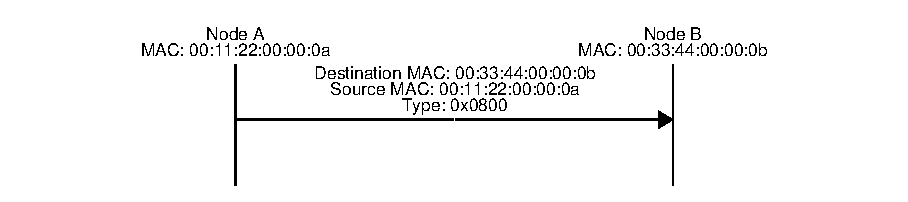
\includegraphics[width=\linewidth]{ethernet_message_unicast.eps}
\end{center}

Ethernet also supports \concept{broadcast} to all nodes in the LAN. In this case, the destination
MAC address must be \otherBase{ff:ff:ff:ff:ff:ff}.
% 
When a device receives a frame, it discards it unless the destination MAC field in the frame
is identical to its own MAC address, or \concept{broadcast}. 

A node will also discard a frame with an unsupported Payload Type (\concept{EtherType}) field. 
% 
If the payload type is supported, it is used to decide what part of the OS receives the message,
\eg, the \concept{IPv4} stack or the \concept{ARP} subsystem.

\begin{exercise} Continuing the example of the figure above, the network card of Node~B receives
a \concept{frame} that begins with the following bytes. Should it be accepted by B?
\begin{center}
\otherBase{00 11 22 00 \quad 00 0a ff ff \quad ff ff ff ff \quad 08 DD \ldots}
\end{center}
\end{exercise}

\begin{exercise}
The following scripts exemplify how to send and receive raw \concept{Ethernet} frames. 
The \concept{client} sends $5$ identical frames of \concept{EtherType} \otherBase{0x1234} and then exits.
The \concept{server} waits until it receives $5$ Ethernet frames of that type (checked in lines 12-13) and then exits.
% 
\begin{itemize}
\item Change the client's MAC address (see page \pageref{sec:layer2:practical}) and interface name with yours.
\item Make the server reject frames not addressed to it.
\item Extend these scripts to implement a simple application with \concept{LAN} capabilities.\\
  Suggested examples:
    \begin{itemize}
    \item A Layer-2 \concept{echo} service that distinguishes between petitions and responses.
    \item A Layer-2 \concept{peer-to-peer} chat that includes the origin's nickname in all messages.
    \item A Layer-2 calculator service that supports basic arithmetic operations\\
      (\inlineCode{+}, \inlineCode{-},\inlineCode{*}, integer division \inlineCode{//}, optionally division \inlineCode{/}).
    \end{itemize}
\item What is missing so that your application can connect to the rest of the \concept{Internet} beyond your \concept{LAN}?
\end{itemize}

\begin{remark}
You will need to run these scripts with privileges, \eg, with \inlineCode{sudo}.
% 
Alternatively, you can permanently add the \texttt{CAP\_NET\_RAW} capabilities
to your python binary with
\begin{center}
\inlineCode{sudo setcap cap_net_raw+ep ./venv/bin/python}.  
\end{center}
% 
After that, you can run \inlineCode{./venv/bin/python script.py} directly without \inlineCode{sudo}.\\[-0.5cm]
\end{remark}
\label{ex:layer2:echo}
\end{exercise}

\begin{center}
\showCode{snippets/ethernetclient.py}
\end{center}

\begin{center}
\showCode{snippets/ethernetserver.py}
\end{center}
